\documentclass{beamer}
\setbeamertemplate{caption}{\insertcaption}
\usepackage{cancel}
\renewcommand\CancelColor{<color command>}
\usefonttheme[onlymath]{serif}
\usepackage{xcolor}
\newcommand\Ccancel[2][black]{\renewcommand\CancelColor{\color{#1}}\cancel{#2}}

\definecolor{bluenewcolor}{RGB}{20,20,100}
\definecolor{greennewcolor}{RGB}{0,100,0}
\definecolor{decisionColor}{HTML}{DEE1B2}
\definecolor{nodeColor}{HTML}{EBFAFF}
\def\mathunderline#1#2{\color{#1}\underline{{\color{black}#2}}\color{black}}
\usetheme{metropolis}           % Use metropolis theme
\title{Master thesis presentation\\
STOCHASTIC APPROACH TO MANY-BODY PROBLEMS}
\date{\today}
\author{Anna Gribkovakaya}
\institute{University of Oslo}
\begin{document}
  \maketitle
  \section{Introduction}
   \begin{frame}{Outline}
   \begin{itemize}
   	\item Many body \textit{Ab initio} methods: deterministic and stochastic
   	\item Many-body problem formulation
   	\item Coupled Cluster Theory
   	\item Coupled Cluster Quantum Monte Carlo
   	\item Results
   	\item Summary
   \end{itemize}
 \end{frame}
   \begin{frame}{Objectives}
	The main objectives:
	\begin{itemize}
 	\item Implement numerical methods to solve the Time Independent Schr\"{o}dinger equation for N electrons
 	\item Study the Homogeneous Electron gas using Coupled Custer approach
 	\item Study the Homogeneous Electron gas using the Coupled Custer Monte Carlo approach
 	\item Compare the two methods
 	\item Develop a code that can be used for other systems (Quantum Dots)
	\end{itemize}
	\end{frame}


  \section{Main Part}
  
  \begin{frame}{Many-body: \textit{Ab initio} quantum many body methods}
  \uncover<1->{Deterministic or Wave Function Methods}
  \uncover<1->{ \begin{itemize}
  		\item Hatree-Fock Method
  		\item Many Body Perturbation Theory
  		\item Full Configuration Interaction 
  		\item Coupled Cluster Method
  \end{itemize}}
   \uncover<2->{Stochastic or Monte Carlo (MC) Methods}
  	  \uncover<2->{	\begin{itemize}
  		\item Variational MC
  		\item Diffusion MC
  		\item Full Configuration MC
  		\item Coupled Cluster MC
  	\end{itemize}}
  \uncover<3->{Density Functional Theory - widely used, but has issues}
   \end{frame}
  \begin{frame}{Many-body: problem formulation}
The Hamiltonian for quantum mechanical system consisting of N particles  can be written as
\begin{equation*}
\hat{H} = -\frac{1}{2}\sum_{i=1}^{N} \nabla_i^2 + \sum_{i<j}^{N}\frac{1}{r_{ij}} - \sum_{i=1}^{N} \hat{V}(r_i),
\end{equation*}
$r_{ij}$  relative distance between the particles, \\
$\hat{V}(r_i)$  potential that represents the system under consideration.\\

Stationary Schr\"{o}dinger equation can be written as:
\begin{equation*}
\hat{H}\Psi_n(\vec{\textbf{R}}) = E_n\Psi_n(\vec{\textbf{R}}),
\end{equation*}
$\vec{\textbf{R}}$ - vector representing both coordinates and spins for all particles.
\begin{equation*}
\vec{\textbf{R}} = \{\vec{R_n}\}= \{(\vec{r}, \sigma)_n\},
\end{equation*}
For fermions the wave function must be antisymmetric:
\begin{equation*}
\Psi_n({\dots, \vec{R}_p , \dots, \vec{R}_q, \dots}) = -\Psi_n({\dots, \vec{R}_q , \dots, \vec{R}_p, \ \dots}),
\end{equation*}
\end{frame}
  \begin{frame}{Many-body: Slater Determinant Space}
  \begin{itemize}
  	\item Slater Determinant (SD) Space is a Hilbert space for fermions 
  	\item Each SD is constructed from $N$ orthonormal single electron
  	wavefunctions
  	
  	\item SD for reference vacuum state :
 
  \begin{equation*}
  |D_0\rangle = \frac{1}{\sqrt{N!}}
  \left| \begin{array}{ccccc} \psi_{1}(x_1)& \psi_{1}(x_2)& \dots & \psi_{1}(x_N)\\
  \psi_{2}(x_1)&\psi_{2}(x_2)& \dots  & \psi_{2}(x_N)\\  
  \vdots & \vdots & \ddots  & \vdots \\
  \psi_{N}(x_1)&\psi_{N}(x_2)& \dots  & \psi_{N}(x_N)\end{array} \right| 
  \end{equation*}
  \item Every  SD is anti-symmetric by construction
   \end{itemize}
  \end{frame}

 \begin{frame}{Many-body: Size of the Slater Determinant Space}
An orthonormal set of 2M spin-orbitals, where N are occupied.
\begin{equation*}
\binom {2M}{N} = \frac{N!}{2M!(2M-N)!}, 
\end{equation*}

For the electron gas:\\
$N$=14, $2M$=3/38	$\rightarrow$ $10^{10}$\\
$N$=14, $2M$=10/246	$\rightarrow$ $10^{22}$\\
$N$=14, $2M$=20/730	$\rightarrow$ $10^{29}$
\end{frame}



\section{Coupled Cluster Theory}

  \begin{frame}{Coupled cluster theory: Exponential ansatz}
	The approximation for wave function for Coupled Cluster is:
	\begin{equation*}
	\Psi_{CC} =  e^{\hat{T}}|D_0\rangle,
	\end{equation*}
	\begin{equation*}
	\hat{T} = \sum_i^{N} \hat{T}_i  = \hat{T}_1 + \hat{T}_2 +\hat{T}_3 + \dots + \hat{T}_N,
	\end{equation*}
	Each excitation operator can be written in terms of creation and annihilation operators:
	\[ 
	\hat{T}_1 = \sum_{i}\hat{t}_i = \sum_{ia}t_{i}^{a} c^\dag_{a}  c_{i}, \text{    } 
	\hat{T}_2 = \sum_{i<j}\hat{t}_{ij}^{ab} = \frac{1}{2!^2}\sum_{ijab}t_{ij}^{ab} c^\dag_{a} c^\dag_{b} c_{j} c_{i}, 
	\]
	\[ 
	\hat{T}_3 = \sum_{i<j<k}\hat{t}_{ijk}^{abc} = \frac{1}{3!^2}\sum_{ijkabc}t_{ijk}^{abc} c^\dag_{a} c^\dag_{b} c^\dag_{c} c_{k}c_{j} c_{i}.
	\,
	\]
	here $i,j,k$ indexes denote the orbitals that are occupied in the reference determinant and $a,b,c$ denote those that are not.
	
\end{frame}




\begin{frame}
\frametitle{Coupled Cluster: Energy and Amplitudes}
Insert the CC approximation for wave function into TISE:
\begin{equation*}
\hat{H}e^{\hat{T}}|D_0\rangle =Ee^{\hat{T}}|D_0\rangle.
\end{equation*}
\begin{equation*}
\langle D_0|\hat{H}|D_0\rangle +  \langle D_0|\hat{H}\hat{T}|D_0\rangle +\langle D_0|\hat{H}\frac{1}{2!}\hat{T}^2|D_0\rangle  = E.
\end{equation*}
In the energy equation is \textit{naturally truncated} after $\hat{T}^2$.
Equations for the amplitudes can be obtained from:
\begin{equation*}
 \langle D_{ij\dots}^{ab\dots}|\hat{H}e^{\hat{T}}|D_0 \rangle = 0.
\end{equation*}
However for practical purposes we are using so-called similarly transformed Hamiltonian and the equations become:
\begin{equation*}
\text{Energy} \Longrightarrow \langle D_0|e^{-\hat{T}}\hat{H}e^{\hat{T}}|D_0\rangle = E,
\end{equation*}
\begin{equation*}
\text{Amplitudes} \Longrightarrow \langle D_{ij\dots}^{ab\dots}|e^{-\hat{T}}\hat{H}e^{\hat{T}}|D_0 \rangle = 0.
\end{equation*}

\end{frame}


\section{Coupled Cluster Quantum Monte Carlo}

\begin{frame}
\frametitle{Coupled Cluster Quantum Monte Carlo}
CCQMC is a Projector Monte Carlo Method and can be introduced as follows: 
\begin{itemize}
	 \uncover<1->{\item Perform Wick rotation to move from time dependent Schr\"{o}dinger equation (TDSE) to TISE
	\begin{equation*}
	-i\hbar \frac{\partial}{\partial t} |\Psi(t)\rangle= \hat{H} |\Psi(t)\rangle \Longrightarrow -\frac{\partial}{\partial \tau} |\Psi(\tau)\rangle= \hat{H} |\Psi(\tau)\rangle,
	\end{equation*}}
	\uncover<2->{\item  Express the wave function for arbitrary $\tau$ with a propagator:
	\begin{equation*}
	|\Psi^{(\tau)}\rangle \propto e^{-\tau \hat{H}}|\Psi^{(\tau = 0)}\rangle,
	\end{equation*}}
	\uncover<3->{\item Assume that initial wave function has nonzero overlap with the ground state of the Hamiltonian:
	\begin{equation*}
	|\Psi_0\rangle = \lim_{\tau \rightarrow \infty} e^{-\tau (\hat{H}-S)}|\Psi^{(\tau = 0)}\rangle,
	\end{equation*}}
\end{itemize}
\end{frame}

\begin{frame}{Coupled Cluster Quantum Monte Carlo}

\begin{itemize}
	\uncover<1->{
		\item Approximate the exponential propagator by repeated application of the linear propagator:
		\begin{equation*}
		|\Psi_0\rangle = \lim_{N \rightarrow \infty} \Big[1 - \delta \tau (\hat{H}-S)\Big]^N |\Psi^{(\tau = 0)}\rangle,
		\end{equation*}}
	\uncover<2->{\item  Introduce wave-function for the imaginary time $\tau + \delta \tau$:
		\begin{equation*}
		|\Psi^{(\tau + \delta \tau)}\rangle = (1 - \delta \tau(\hat{H}-S))| \Psi^{(\tau)}\rangle.
		\end{equation*}}
	
	\uncover<3->{\item Insert a coupled cluster approximation for the wave function and project equation on the excited determinant $D_{\{\boldsymbol{i}\}}$:}
	\uncover<3->{\begin{align*}
		\langle D_{\{\boldsymbol{i}\}}|e^{\hat{T}}D_0\rangle = \langle D_{\{\boldsymbol{i}\}}|e^{\hat{T}}D_0\rangle - \delta \tau \langle D_{\{\boldsymbol{i}\}}|(\hat{H}-S)e^{\hat{T}}|D_0\rangle,
		\end{align*}}
\end{itemize}

\end{frame}


\begin{frame}
\frametitle{Coupled Cluster Quantum Monte Carlo}
\begin{itemize}
\uncover<1->{\item Express the RHS of the above equation in terms of amplitudes:}
\uncover<1->{\begin{equation*}
	\langle D_{\boldsymbol{i}}|e^{\hat{T}^{(\tau)}}D_0\rangle = t_{\boldsymbol{i}}^{(\tau)} + \mathcal{O}(\hat{T}^2),
	\end{equation*}}
\uncover<2->{\item Derive the equation for the amplitudes for $\tau+\delta\tau$: 
	\begin{equation*}
	t_{\{\boldsymbol{i}\}}^{(\tau+\delta\tau)}  \only<3>{+\mathcal{O}(\hat{T}^2)\phantom{2}}\only<4>{+\Ccancel[red]{\mathcal{O}(\hat{T}^2)}\phantom{2}}\only<5>{} = t_{\{\boldsymbol{i}\}}^{(\tau)}  \only<3>{+\mathcal{O}(\hat{T}^2)\phantom{2}}\only<4>{+\Ccancel[red]{\mathcal{O}(\hat{T}^2)}\phantom{2}}\only<5>{} - \delta \tau \langle D_{\{\boldsymbol{i}\}}|(\hat{H}-S)e^{\hat{T}}|D_0\rangle,
	\end{equation*}}
\uncover<5->{\item Rewrite it to obtain CCQMC population dynamics equation:
	\begin{equation*}
	\frac{\delta t_{\{\boldsymbol{i}\}}}{\delta\tau} = -\langle D_{\{\boldsymbol{i}\}}|(\hat{H}-S)e^{\hat{T}}|D_0\rangle,
	\end{equation*}}
	\uncover<6->{This looks very similar to the diffusion equation!}	
\end{itemize}
\end{frame}

\begin{frame}
\frametitle{Coupled Cluster Quantum Monte Carlo}
Diffusion equation with the first-order rate term for chemically reactive systems:
\begin{equation*}
\frac{\partial C}{\partial t} = D\nabla^2 C - kC,
\end{equation*}
\uncover<2->{Diffusion Monte Carlo  Schr\"{o}dinger Equation :}
\uncover<2->{\begin{equation*}
	-\frac{\partial}{\partial \tau} |\Psi(\tau)\rangle= (\only<2>{\frac{1}{2}\nabla^2}  - \only<2>{(\hat{V} -E_0)}) |\Psi(\tau)\rangle,
	\end{equation*}}
\end{frame}


\begin{frame}
\frametitle{Coupled Cluster Quantum Monte Carlo}
\begin{equation*}	
\frac{\delta t_{\{\boldsymbol{i}\}}}{\delta\tau} = -\langle D_{\{\boldsymbol{i}\}}|(\hat{H}-S)e^{\hat{T}}|D_0\rangle,
\end{equation*}
Amplitudes $\rightarrow$ walkers $\equiv$ {\color{red}excips}
\begin{equation*}	
t_{\boldsymbol{i}} \propto N_{\boldsymbol{i}} = \sum_\alpha s_\alpha \delta_{{\boldsymbol{i}},{\boldsymbol{i}}_\alpha} ,\ \ \ |D_{\boldsymbol{i}}\rangle = \hat{c}_{\boldsymbol{i}}|D_0\rangle,
\end{equation*}
Excip $\alpha$ is located on a determinant ${\boldsymbol{i}}_\alpha$ and has sign $s_\alpha = \pm 1$.
\begin{equation*}	
N_{ex} = \sum_{\boldsymbol{i}} |N_{\boldsymbol{i}}|, 
\end{equation*}
\only<1>{\begin{equation*}
\Psi_{cc} = \big[1 + \sum_{\boldsymbol{i}} t_{\boldsymbol{i}}\hat{a}_{\boldsymbol{i}} + \frac{1}{ 2!}\sum_{\boldsymbol{ij}} t_{\boldsymbol{i}} t_{\boldsymbol{j}} \hat{a}_{\boldsymbol{i}} \hat{a}_{\boldsymbol{j}} + \frac{1}{ 3!}\sum_{\boldsymbol{ijk}}t_{\boldsymbol{i}} t_{\boldsymbol{j}} t_{\boldsymbol{k}} \hat{a}_{\boldsymbol{i}} \hat{b}_{\boldsymbol{j}} \hat{a}_{\boldsymbol{k}} + ...  \big]|D_0\rangle.
\end{equation*}}
\end{frame}


\section{Results}
\begin{frame}
\frametitle{Benchmarking}
\begin{table}[h]
	\centering
	%\captionsetup{width=.8\textwidth}
	\caption{\tiny CCD(deterministic) results for $14$ electrons. Mixing parameter $\alpha=0.8$ for Miller's results, and $\alpha=0.3$ for our results. All energies are presented in Hartree units.} \label{tab:CCDcompar}
	\tiny  %%  command to change the font size
	\begin{tabular}{rrll}
		$r_s$ & States & $\Delta E_{CCD}$ \footnote{\tiny Quantum Mechanical Studies of Infinite Matter by the Use of Coupled-Cluster Calculations, with an Emphasis on Nuclear Matter. Sean Bruce Sangolt Miller. 2017}  & $\Delta E_{CCD}$\\
		\hline
		\hline
		1.0 & 54 & -0.3178228436889338 & -0.3178230699319593  \\
		1.0 & 66 & -0.3926965898061968 & -0.3926968074770886  \\
		1.0 & 114 & -0.4479105961757175 & -0.4479109389185165  \\
		1.0 & 162 & -0.4805572589306421 & -0.4805570782443642  \\
		1.0 & 186 & -0.4855229317521320 & -0.4855227418241649  \\
		1.0 & 246 & -0.4929245740023971 & -0.4929243692209991  \\
		1.0 & 294 & -0.4984909094066806 & -0.4984906939593084  \\
		1.0 & 342 & -0.5019526761547777 & -0.5019524529049425  \\
		1.0 & 358 & -0.5025196736076414 & -0.5025194488388953  \\ \hline
		0.5 & 114 & -0.5120153541478306 & -0.5120152296730573  \\
		0.5 & 342 & -0.5729645498903680 & -0.572964399507112   \\ \hline    
		2.0 & 114 & -0.3577968843144996 & -0.3577955282575226  \\
		2.0 & 342 & -0.4014136184665558 & -0.4014117905655014  \\
	\end{tabular}
\end{table}
%\begin{thebibliography} 
%	\bibitem[Quantum Mechanical Studies of Infinite Matter by the Use of Coupled-Cluster Calculations, with an Emphasis on Nuclear Matter]{abc}
%\end{thebibliography}

\end{frame}

%\begin{frame}
%\frametitle{Benchmarking}
%\begin{figure}[ht!]
%	\centering
%	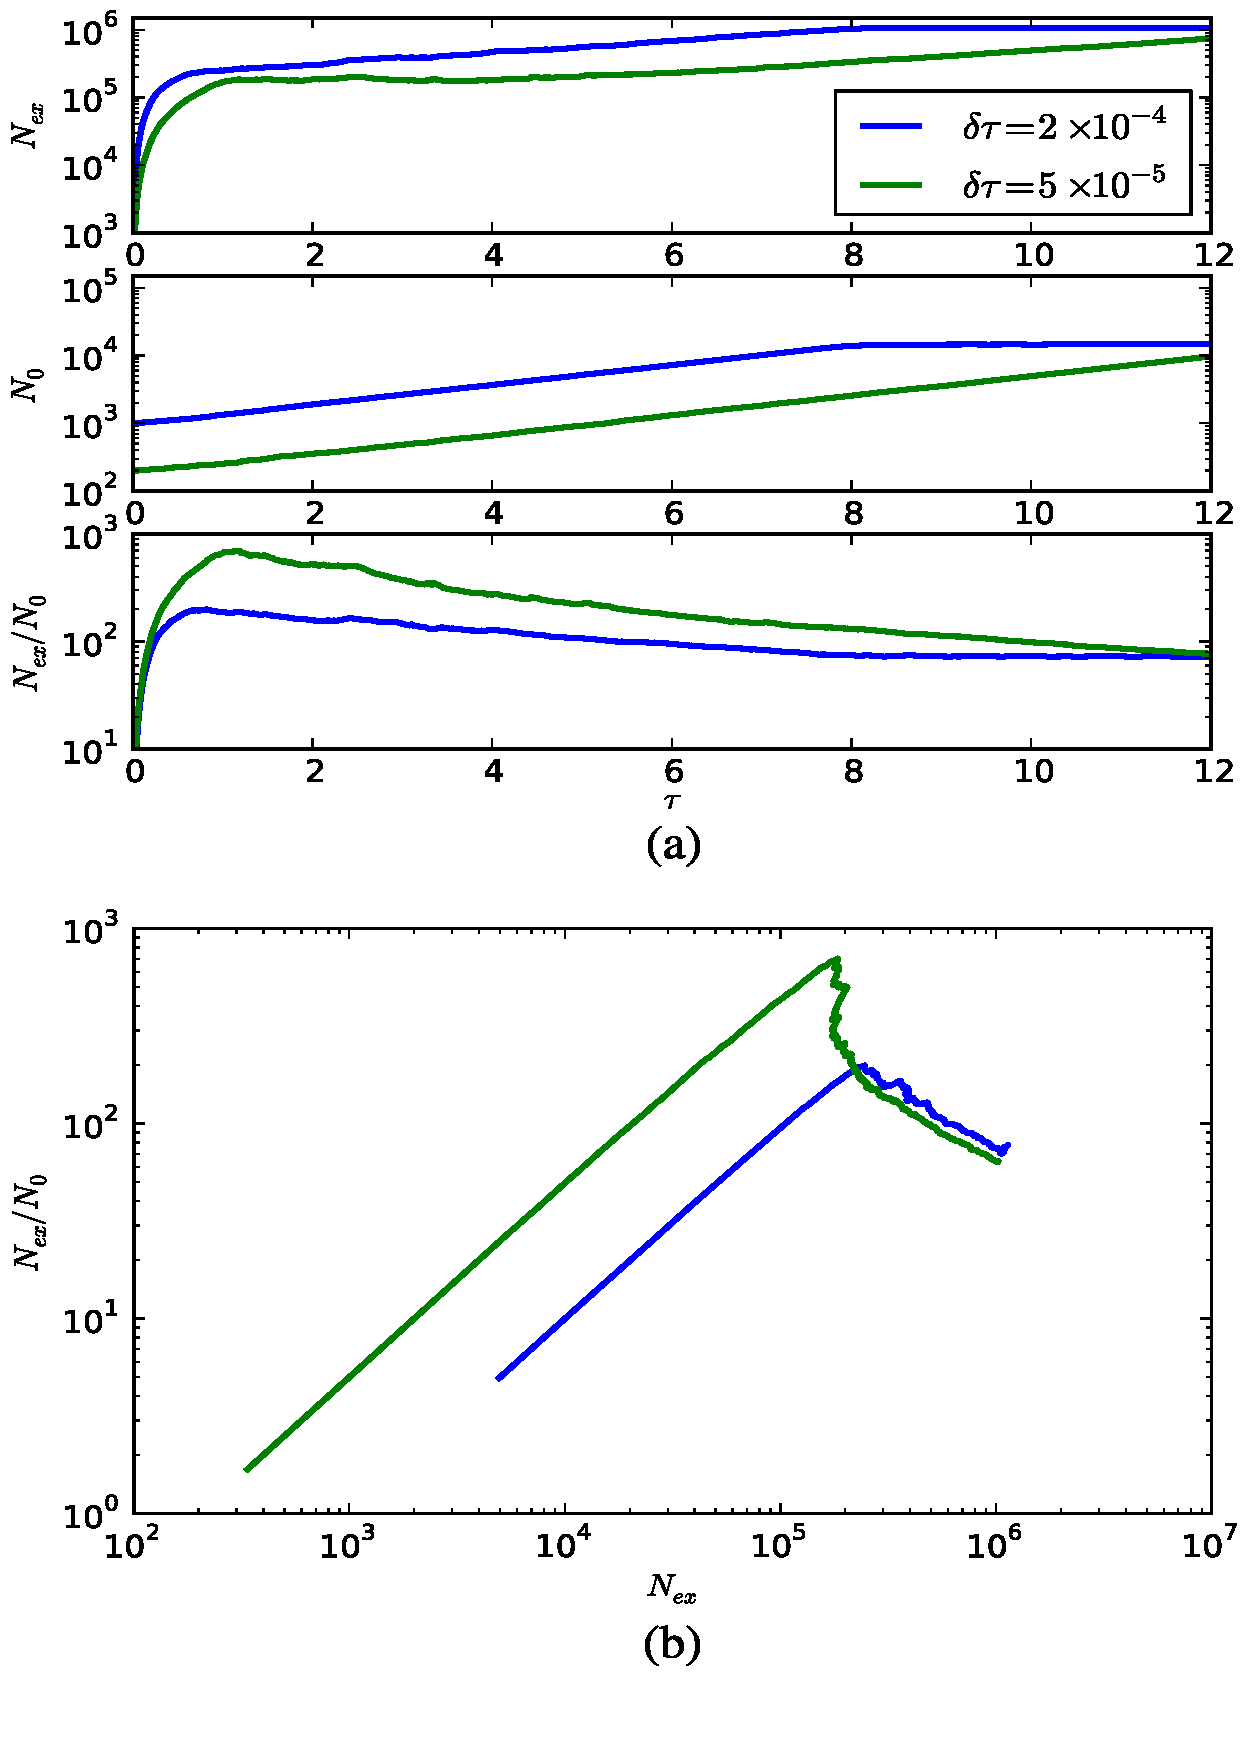
\includegraphics[scale=0.30]{thomEG}
%	\caption{ }
%	%\label{}
%\end{figure}
%\end{frame}
\begin{frame}
\frametitle{Population dynamics}

\begin{columns}
\begin{column}{0.60\textwidth}
	\begin{center}
		\begin{figure}
			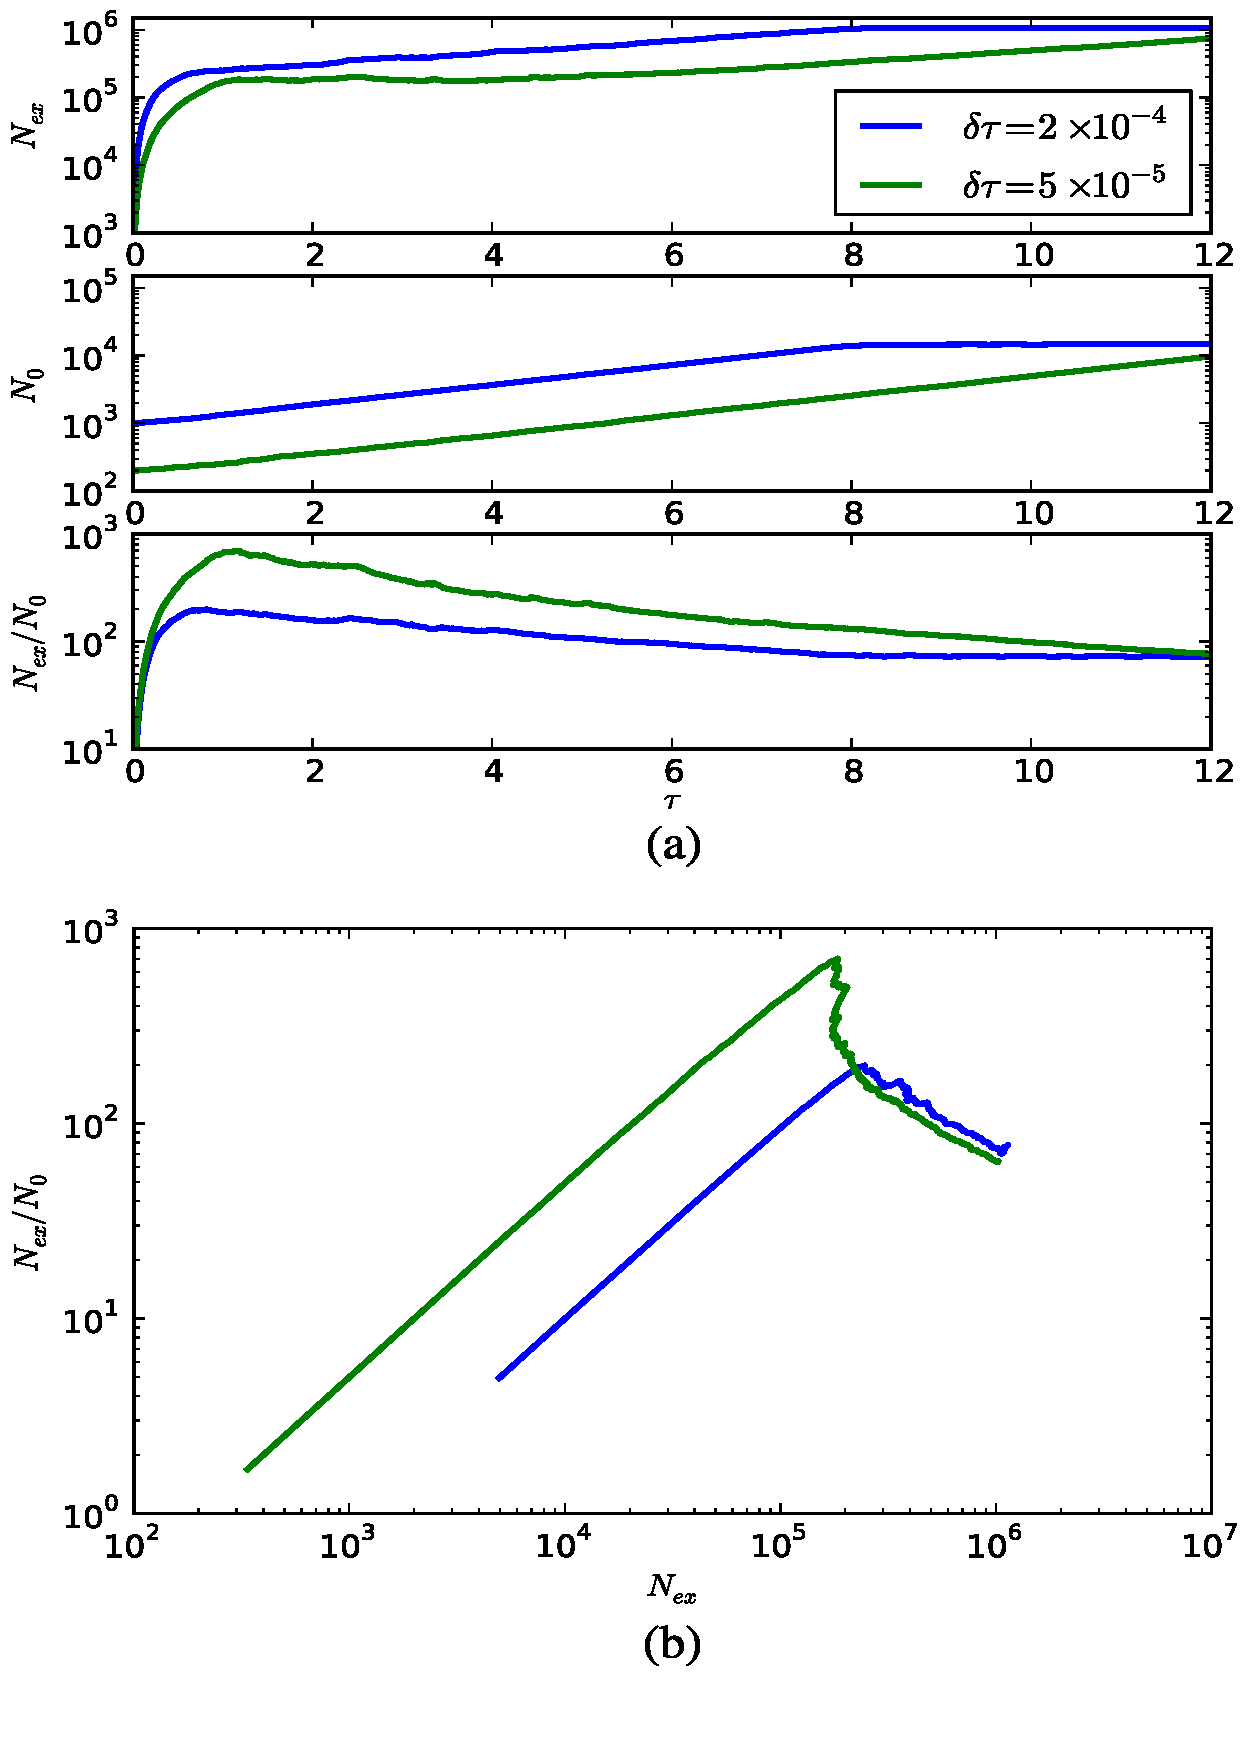
\includegraphics[scale=0.20]{thomEG}
		\end{figure}
	\end{center}
\end{column}
\begin{column}{0.40\textwidth}
	\tiny Ne CCSDTQ calculations starting with different initial
	particle numbers at the reference and different timesteps. (a): With a carefully
	chosen low timestep and initial population, a plateau is visible. An increased
	timestep and initial population overshoot the plateau but have a shoulder.
	The lower panel shows a maximum of the particle ratio at the position of the
	shoulder and plateau. (b): "Shoulder plots" allow shoulder height to be read off
	easily.  \footnote{\tiny James S. Spencer and Alex J. W. Thom. “Developments in\\ Stochastic
		Coupled Cluster Theory: The Initiator Approximation\\ and Application to the
		Uniform Electron Gas”.\\ The Journal of Chemical Physics 144.8 (Feb.
		2016)}
\end{column}
\end{columns}	
\end{frame}

\begin{frame}
\frametitle{Population dynamics}

\begin{columns}
\begin{column}{0.48\textwidth}
\begin{center}
	\begin{figure}
		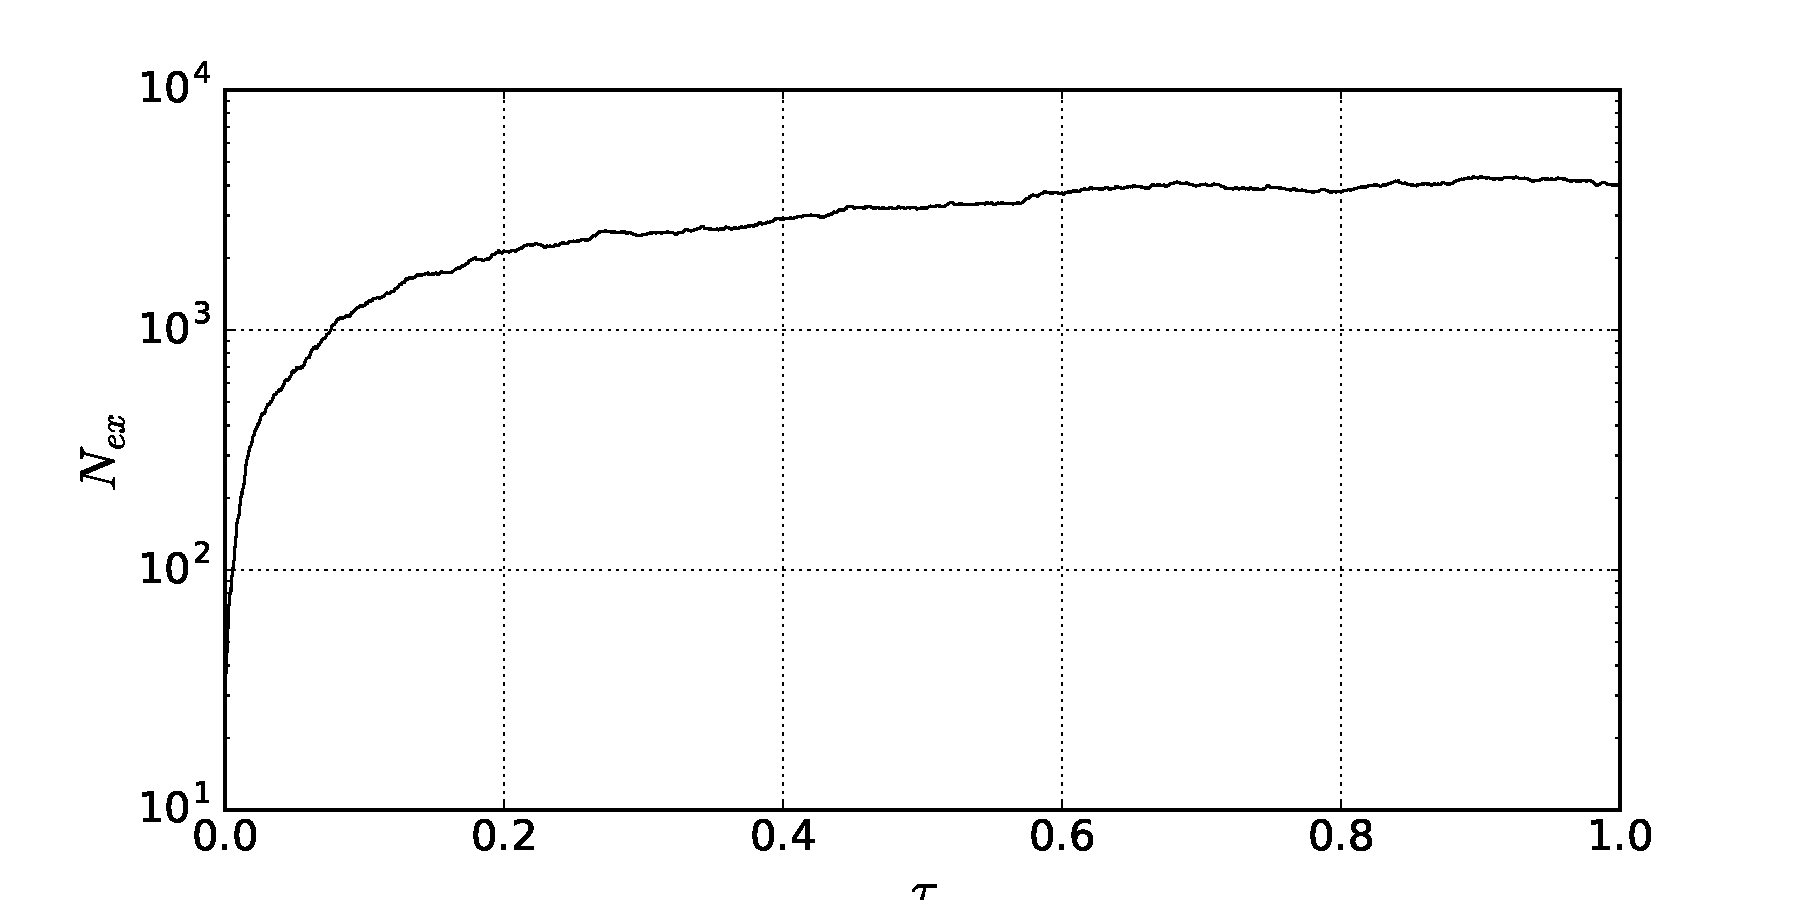
\includegraphics[scale=0.20]{Nex2000new}
	\end{figure}
\end{center}
\end{column}
\begin{column}{0.48\textwidth}
\begin{center}
	\begin{figure}
		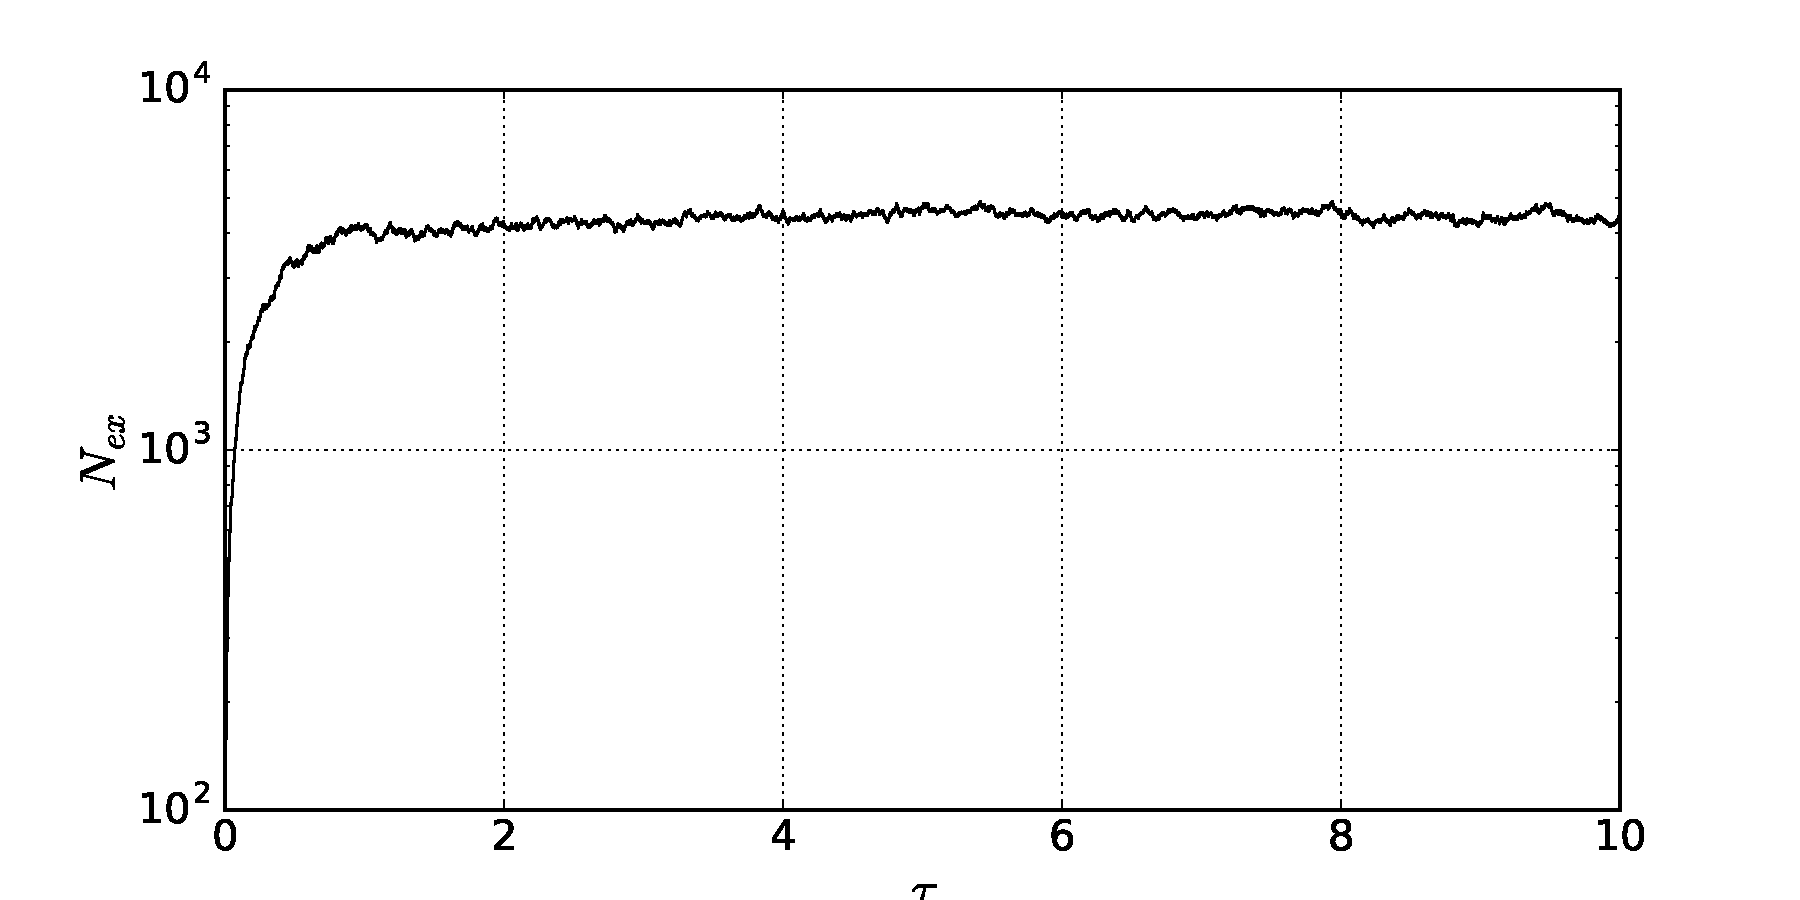
\includegraphics[scale=0.20]{Nex20000}
	\end{figure}
\end{center}
\end{column}
\end{columns}
\tiny The population dynamics of the excited space for 14 electrons and 54 basis functions. $r_s=0.5$, $\delta \tau=0.0005$(left).
The population dynamics of the excited space for 14 electrons and 54 basis functions with $r_s=0.5$, $\delta \tau=0.0005$ and the population control enabled after $5\cdot 10^3$ iterations. Dampening parameter is $\gamma = 0.05$. The energy shift $S$ is tuned every five iterations.(right) 	
\end{frame}

\begin{frame}
\frametitle{Population dynamics}
\begin{figure}[ht!]		
\centering
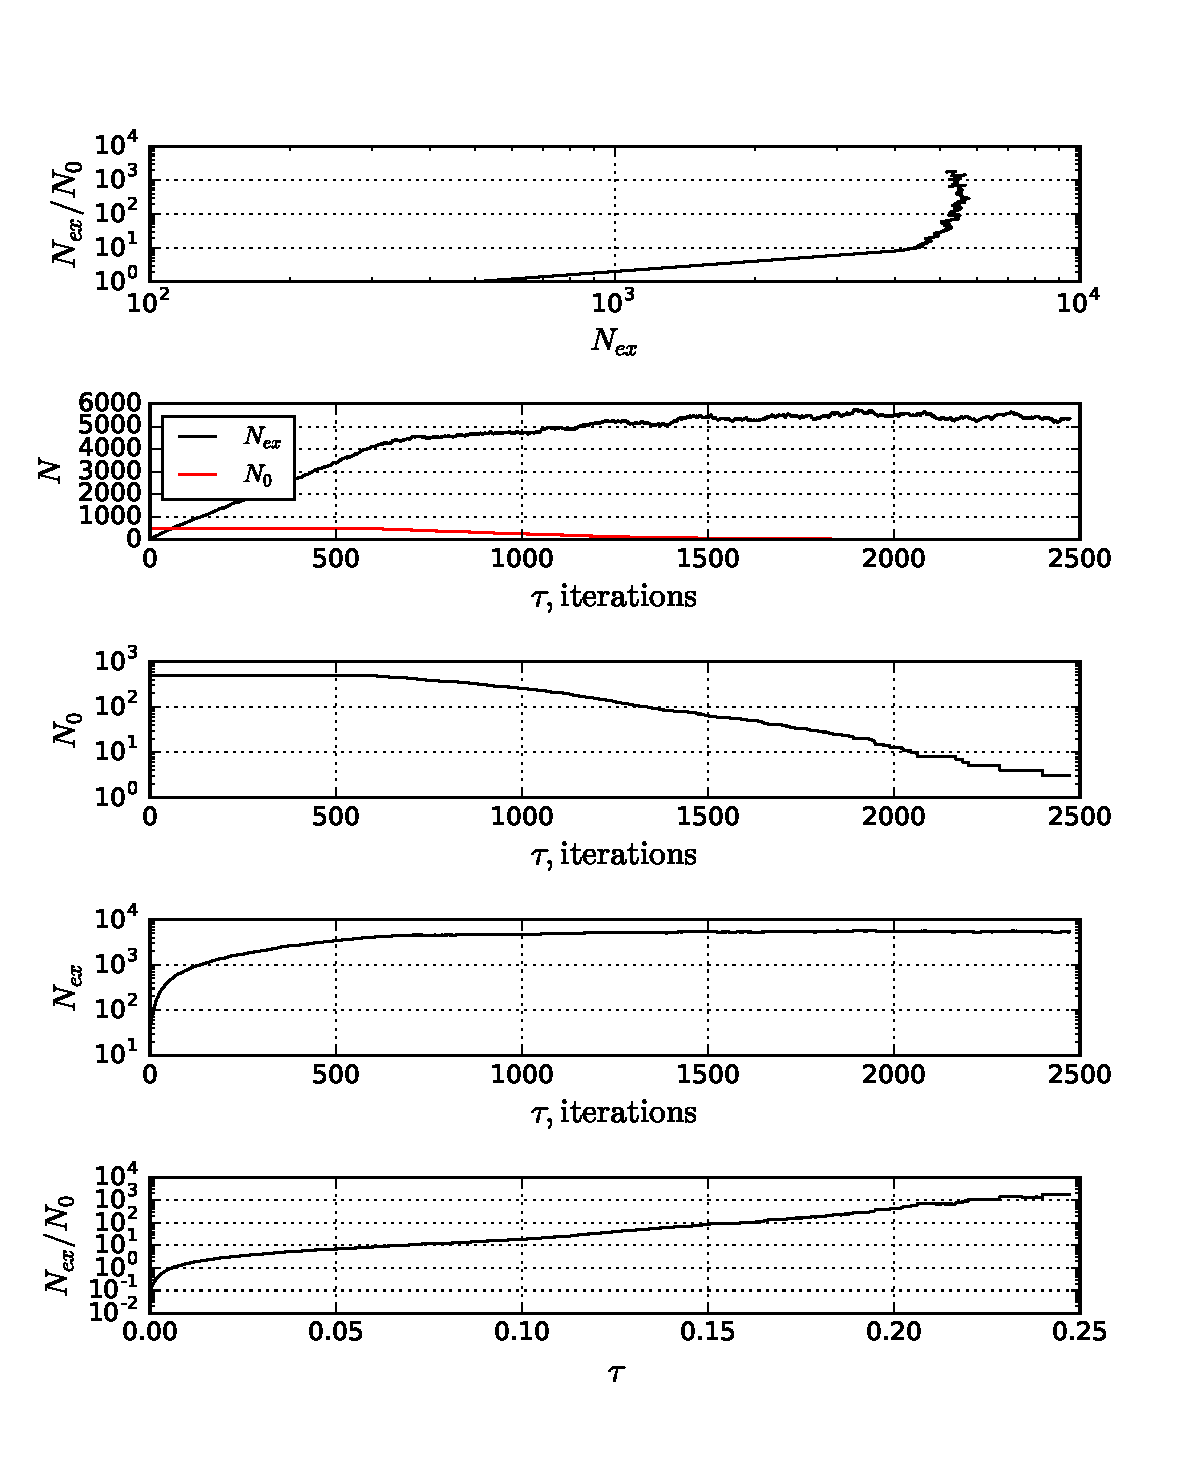
\includegraphics[scale=0.30]{deathN0}
\caption{ }
\label{fig:thomEG}
\end{figure}
\end{frame}


\begin{frame}
\frametitle{CBS energies}
\begin{table}[h]
\centering
\caption{\tiny Summary of complete basis set extrapolated results for the correlation energy of the 14 electron uniform electron gas in hartree. $r_s = 1.0$} \label{tab:CCDQMC}
\tiny  %%  command to change the font size
\begin{tabular}{ll}
$-$ &  $\Delta E_{CCD}$ \\
\hline
\hline
dCCD & -0.514204 \\
dCCD\footnote{\tiny J. J. Shepherd, A. Grüneis, G. H. Booth, G. Kresse, and A. Alavi, Phys. Rev. B 86, 035111 (2012)} & -0.5152(5) \\
\hline
qCCSD\footnote{\tiny Verena A. Neufeld and Alex J. W. Thom. "A Study of the Dense Uniform Electron Gas with High Orders of Coupled Cluster". The Journal of Chemical Physics 147.19 (Nov. 2017)} & -0.51450(9) \\
qCCSDT$^3$ & -0.5307(2) \\
qCCSDTQ$^3$ & -0.5307(2) \\			
\hline
FCIQMC\footnote{\tiny J. J. Shepherd, G. H. Booth, and A. Alavi, J. Chem. Phys. 136, 244101 (2012)} & -0.5325(4) \\
\hline     
\end{tabular}
\end{table}
%\begin{thebibliography} 
%	\bibitem[Quantum Mechanical Studies of Infinite Matter by the Use of Coupled-Cluster Calculations, with an Emphasis on Nuclear Matter]{abc}
%\end{thebibliography}

%\footnote{\tiny Verena A. Neufeld and Alex J. W. Thom. "A Study of the Dense Uniform Electron Gas with High Orders of Coupled Cluster". The Journal of Chemical Physics 147.19 (Nov. 2017)}


\end{frame}


\section{Conclusion}

\begin{frame}
\frametitle{Conclusion}
\begin{itemize}
\item We have developed a CCD code capable of handling relatively large system sizes. 
\item The code was developed with generality in mind, and can be applied for other systems.
\item Our CCD solver reproduced published results for the homogeneous electron gas.
\item Deterministic implementation provides a significant benchmark information for the further development of the code for the stochastic CCQMC.
\end{itemize}
\end{frame}

\begin{frame}
\frametitle{Conclusion}
\begin{itemize}
\item We have developed a CCD code for the CCQMC algorithm.
\item The population of the reference state plays one of the majors roles for the CCQMC algorithm.
\item Transitionally invariant systems are not an optimal choice as a test system for the CCQMC method. At least at low truncation levels.
\end{itemize}
\end{frame}
\section{Future work}
\begin{frame}
\frametitle{Future work}
\begin{itemize}
\item There is a limited theoretical framework for the CCQMC
sign problem.
\item Further research might investigate different sampling schemes.
\item Optimization techniques such as initiator approximation might be a very important topic for future work.
\item The optimization of the implementation both numerically and algorithmically.
\end{itemize}
\end{frame}

\end{document}